%\chapter{Fase di studio e analisi del lavoro esistente}
\section{Fase di studio e analisi del lavoro esistente}
\subsection{Introduzione}
Lo scopo di questa relazione è quello di fornire un punto di riferimento per la riproduzione di approcci per la modellazione digitale di capi di abbigliamento.
Nei prossimi capitolo saranno descritti i seguenti argomenti: formalizzazione del problema, usando mesh poligonali; descrizione degli approcci presenti in letteratura che stimano il volume del corpo umano e la mesh poligonale corrispondente ai vestiti (1) partendo da immagini 2D, e (2) partendo da scansioni volumetriche (3D); un'analisi approfondita del modello con il trade-off migliore, insieme a delle linee guida per la riproduzione del metodo.
%In questo paragrafo viene spiegato brevemente il percorso di analisi del lavoro esistente riguardo la modellazione virtuale di vestiti su mesh tre-dimensionali.

\paragraph{Mesh}
Una mesh poligonale è la partizione di una superficie continua in celle poligonali, come triangoli, quadrilateri, ecc.
Più formalmente, una mesh \( M \) può essere definita come una \emph{tupla} \( (V, K) \), dove 
\[
V = \{ \mathbf{v}_i \in \mathbb{R}^3 \mid i = 1, \ldots, N_v \}
\]
è l'insieme dei vertici del modello (punti in \( \mathbb{R}^3 \)) e \( K \) contiene l'\emph{adjacency information}, ovvero come i vertici sono connessi per formare gli spigoli e le facce della mesh.

\paragraph{Review}
Inizialmente sono stati studiati articoli che riguardano l’estrazione di mesh del corpo umano partendo da immagini e video, ma per seguire questa strada c’è bisogno prima di stimare la forma del corpo del soggetto in esame e poi procedere all’estrazione delle mesh dei singoli vestiti separate da quella del corpo stesso. Per questa ragione si è passati poi alla ricerca di dataset contenenti scansioni 3D e articoli di lavori correlati riguardanti la stratificazione di mesh inerenti a corpo umano nudo ed indumenti indossati.

Tra i lavori ritenuti interessanti troviamo un self-supervised framework (\href{https://openaccess.thecvf.com/content/ICCV2021/papers/Sanyal_Learning_Realistic_Human_Reposing_Using_Cyclic_Self-Supervision_With_3D_Shape_ICCV_2021_paper.pdf}{SPICE}) \cite{sanyal2021learning} che, partendo dall’immagine di una persona, è in grado di generare una nuova immagine di tale soggetto in una posa target, raggiungendo performance dello stato dell’arte sul DeepFashion dataset, con prestazioni migliori rispetto a metodi non supervisionati e simili allo stato dell’arte di metodi supervisionati. SPICE, inoltre, genera video partendo da una singola immagine data in input ed una sequenza di pose, nonostante sia stato addestrato solo su immagini statiche.

\medskip

\subsection{Approcci 2D}

Volendo partire da immagini 2D per predire il volume del corpo umano svestito e la mesh dei vestiti indossati, sono stati analizzati i seguenti articoli:

\begin{itemize}
\item End-to-end Recovery of Human Shape and Pose,
\item Moulding Humans,
\item BodyNet,
\item Parsing clothing in fashion photograph,
\item Multi-garment Net.

\end{itemize}


\subsubsection{End-to-end Recovery of Human Shape and Pose}

In “End-to-end Recovery of Human Shape and Pose” \cite{kanazawa2018end} viene fatta una Human Mesh Recovery (HMR), viene ricostruita cioè una mesh 3D di un corpo umano, partendo dalle immagini RGB del dataset Human3.6M.
Da una GAN vengono generati parametri relativi a posa, shape e camera.
Questo sembrerebbe estrarre meglio il corpo senza vestiti rispetto a BodyNet e Moulding humans, ma non è sempre assicurato che la forma corrisponda alla realtà (ad esempio, per quanto riguarda foto di donne incinta, nella costruzione della forma 3D viene eliminata la pancia perché confusa con gli abiti). Questo perché la rete si occupa principalmente di generare una shape che sembri reale, piuttosto che ottenerne una corrispondente al corpo originale ritratto in foto.
Dunque necessiterebbe di migliorie quali l’aggiunta di tipi di forme del corpo non previste nel lavoro originale.
Il dataset Human3.6M, mette a disposizione 3.6 milioni di immagini di persone e le corrispondenti pose e mesh, acquisite mediante quattro camere digitali. I dati sono organizzati in quindici movimenti di training, tra i quali camminare con vari tipi di asimmetrie (per esempio, camminare con una mano nella tasca, o con una borsa sulla spalla), pose di persone in attesa, sedute o sdraiate, ecc. Tali movimenti sono stati eseguiti da undici attori professionisti, sei uomini e cinque donne, scelti per coprire un indice di massa corporea (BMI) da 17 a 29, in modo da fornire una moderata variabilità per quanto riguarda la forma del corpo e i diversi movimenti.

\newpage

\subsubsection{Moulding Humans}

“Moulding Humans” (2019 - \url{https://openaccess.thecvf.com/content_ICCV_2019/papers/Gabeur_Moulding_Humans_Non-Parametric_3D_Human_Shape_Estimation_From_Single_Images_ICCV_2019_paper.pdf}) usa immagini 2D e, tramite una GAN genera delle mappe di profondità che sono usate per ricostruire la forma della persona.
Stima le profondità dalla foto senza fare troppa distinzione tra clothed e non clothed, a differenza del HMR.


\subsubsection{BodyNet}
La rete neurale proposta, BodyNet (\url{https://arxiv.org/abs/1804.04875}), è una rete neurale in grado di produrre una stima della forma del corpo volumetrico, prendendo in input una singola immagine. Si tratta di una rete addestrabile end-to-end che beneficia di (i) una loss volumetrica 3D, (ii) una loss di riproiezione multi-view e (iii) supervisione intermedia della posa 2D, della segmentazione delle parti del corpo 2D e della posa 3D. Per la evaluation del metodo, viene adattato il modello SMPL all’output della rete BodyNet che prende in ingresso i dataset SURREAL e Unite the People. Tale rete è composta, dunque, da quattro moduli: (i) un modulo per l’estrazione della posa 2D, (ii) un modulo per estrarre una possibile segmentazione 2D, dopodichè (iii) i due moduli precedenti vengono combinati insieme all'immagine originale, permettendo di ottenere la posa 3D, e, infine, (iv) usando i 4 ingressi descritti precedentemente si ottiene in output la forma volumetrica, che viene usata come riferimento per ottimizzare il modello SMPL (che ottiene la unclothed shape).

\subsubsection{Parsing clothing in fashion photograph}
Nonostante l’abbigliamento determini gran parte della shape di una persona, ci sono stati relativamente pochi tentativi di riconoscimento computazionale dei capi di abbigliamento: ci si è focalizzati principalmente sull’identificazione delle parti del corpo, divise in superiore ed inferiore, per poi rappresentare l’abbigliamento come una deformazione del contorno del corpo sottostante. Di recente sono stati fatti dei tentativi per considerare i capi di abbigliamento come attributi semantici di una persona, ma solo per quanto riguarda un numero limitato di indumenti (come t-shirt, jeans, pantaloncini, ecc).
A differenza di tali approcci, in “Parsing clothing in fashion photograph” si cercano di stimare in maniera precisa le aree della superficie relative ad un’ampia lista di possibili capi indossati da un soggetto ( come scarpe, cappello, cintura, calzini, ecc).

\begin{figure}[ht!]
  \centering
  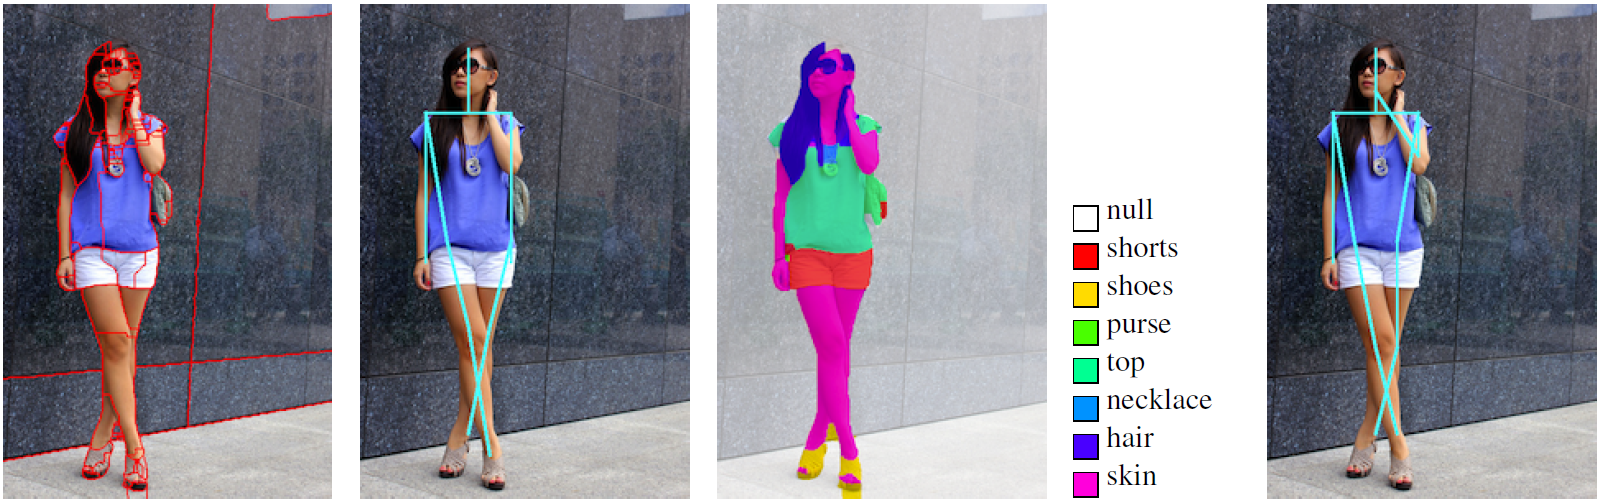
\includegraphics[scale=0.4]{Images/IntroductionPic/parsingclothing.png}
  \caption{(a) Superpixels (b) Stima della posa (c) Segmentazione dei capi di abbigliamento (d) Stima della posa finale }
  \label{fig:SMPL2}
\end{figure}
Per tale analisi, viene utilizzato un dataset che comprende 158’235 foto, con relativa descrizione, stile ed occasione per la quale l’outfit è stato indossato, ed un modello di riconoscimento che permette la segmentazione dei singoli capi di abbigliamento. Per semplificare tale processo, si assume che ogni capo di abbigliamento corrisponde ad una particolare area della superficie del corpo. In questo studio, la posa è fondamentale, in quanto può causare occlusioni importanti e di conseguenza complicare il riconoscimento degli abiti, per tale ragione viene effettuata anche una stima della posa a partire dall’immagine.

\medskip

\subsubsection{Multi-Garment Net}

In “Multi-Garment Net: Learning to Dress 3D People from Images” (\url{https://arxiv.org/pdf/1908.06903.pdf}) viene introdotta la rete multi-indumento (MGM, Multy-Garment Network), ovvero il primo modello in grado di posizionare dei layers esterni di vestiti (con mesh esclusive) direttamente sopra all’immagine data in input.
Come si può vedere nella figura sottostante, questa nuova rappresentazione permette il pieno controllo sulla forma del corpo, sulla struttura e geometria dell’abbigliamento e apre le porte ad una vasta gamma di applicazioni VR/AR, intrattenimento, cinematografiche e virtual try-on.

\begin{figure}[ht!]
  \centering
  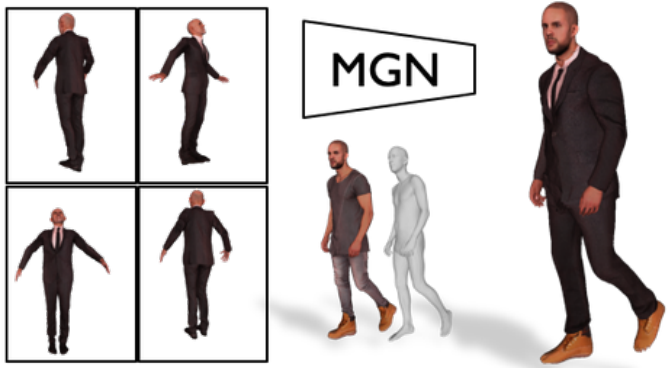
\includegraphics[scale=0.7]{Images/SizerPic/MultyGarmetNet.png}
  \caption{Da sinistra a destra: immagini dal soggetto sorgente, corpo dal
soggetto target, target vestito con indumenti originali. Da uno o
più immagini, MGN può ricostruire la forma del corpo e ciascuna di esse
i capi separatamente. Possiamo trasferire i capi previsti a
un corpo nuovo che include geometria e texture.}
    \label{fig:MultyGarmetNet}
\end{figure}

\newpage
Per raggiungere questo livello di controllo, MGM affronta due sfide principali:

\begin{enumerate}
\item apprendimento di un modello per ogni abito da scansioni tridimensionali di persone vestite
\item imparare a ricostruire tali modelli dalle immagini stesse
\end{enumerate}

\medskip

Per fare ciò, viene definito un insieme discreto di templates di abbigliamento (in base alle varie categorie: maglie lunghe/corte, pantaloni lunghi/corti e cappotti) e viene registrato, per ogni categoria, un singolo template per ciascuna delle istanze delle scansioni che vengono automaticamente segmentate in parti di vestito e pelle.
Poiché la geometria dell'indumento varia in modo significativo all'interno di una categoria (ad es. forme diverse, lunghezze delle maniche), per prima cosa viene ridotto al minimo la distanza tra il modello ed i bordi della scansione, cercando di preservare il laplaciano della superficie del modello.
In questo modo viene compilato un guardaroba digitale di veri capi 3D indossabili dalle persone (come mostrato sotto in Figura).

\medskip

\begin{figure}[ht!]
  \centering
  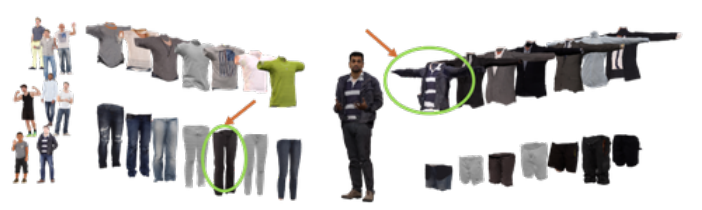
\includegraphics[scale=0.6]{Images/SizerPic/Sizer3.png}
  \caption{Viene utilizzato l'approccio di registrazione multi-mesh proposto per registrare i capi presenti nelle scansioni (a sinistra) su
modelli di indumenti fissi. Questo permette di costruire un guardaroba digitale e vestire soggetti arbitrari (al centro) selezionando i capi (segnati)
dall'armadio.}
    \label{fig:Sizer3}
\end{figure}

\medskip

A partire da tali registrazioni, viene introdotto un modello PCA basato sui vertici degli abiti.
Siccome gli indumenti sono associati (naturalmente) al sottostante modello SMPL, è possibile usarli su diverse morfologie del corpo e riposizionarli usando SMPL.

\medskip

Dal guardaroba digitale, MGM è addestrato a prevedere, data 
\begin{itemize}
\item una o più immagini della persona
\item posa del corpo
\item parametri della forma corporea
\end{itemize}

\medskip

I coefficienti PCA di ciascuno dei capi oltre che ad un “campo di variazione” sopra al modello PCA che codifica i dettagli dell’abbigliamento.
Al momento del test, vengono perfezionate queste stime bottom-up
con un nuovo obiettivo top-down che costringe gli indumenti e la pelle proiettati ad analizzare la segmentazione semantica dell'input.

\medskip

\begin{figure}[ht!]
  \centering
  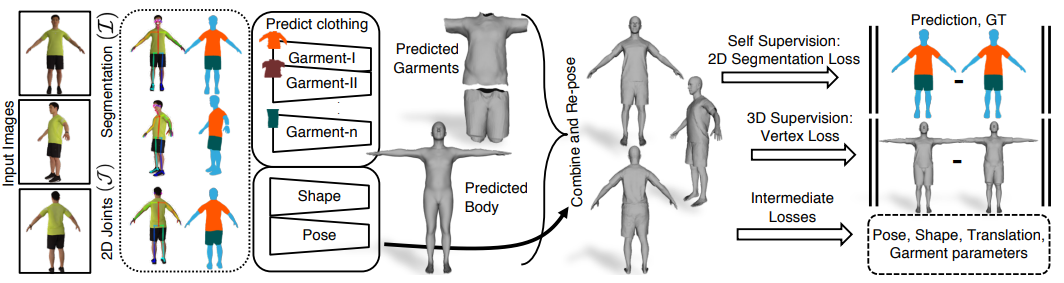
\includegraphics[scale=0.5]{Images/SizerPic/Sizer4.png}
  \caption{Dato un piccolo numero di frame RGB (attualmente 8), vengono pre-calcolate immagini segmentate semanticamente
$(I)$ e Giunti $2D (J)$. Il Multi-Garment Network (MGN), prende ${I,J}$ come input e deduce gli indumenti separabili e il sottostante
forma umana in una posa canonica. Queste previsioni vengono riposte usando le previsioni di posa per fotogramma. Viene fornito la  MGN con una combinazione di Supervisione 2D e 3D. La supervisione 2D può essere utilizzata per il perfezionamento online al momento del test.}
    \label{fig:Sizer4}
\end{figure}

\newpage

Per apprendere un modello in grado di prevedere la forma del corpo e la geometria degli indumenti direttamente dalle immagini è necessario processare un dataset di 356 scansioni di persone con un’ampia varietà di vestiti, pose e morfologie.

\medskip

Per quanto riguarda la pre-processazione dei dati abbiamo:
\begin{itemize}
\item registrazione SMPL alle scansioni
\item scansione e segmentazione del corpo
\item registrazione del template
\end{itemize}

\medskip

Per ogni scansione viene ottenuta la forma del corpo al di sotto degli abiti e gli indumenti della persona, registrati in uno dei 5 modelli d’abbigliamento:
\begin{itemize}
\item camicia
\item t-shirt
\item cappotto
\item pantaloni corti
\item pantaloni lunghi
\end{itemize}

\medskip

I modelli di abbigliamento sono definiti come regioni sulla superficie SMPL dove la forma originale segue quella del corpo umano ma si deforma adattandosi ad ogni istante di scansione avvenuta dopo la registrazione.

\medskip

In questo modo viene formata (sotto training process) la MGN per stimare la forma del corpo e gli indumenti da una o più immagini di una persona.

\medskip

\begin{figure}[ht!]
  \centering
  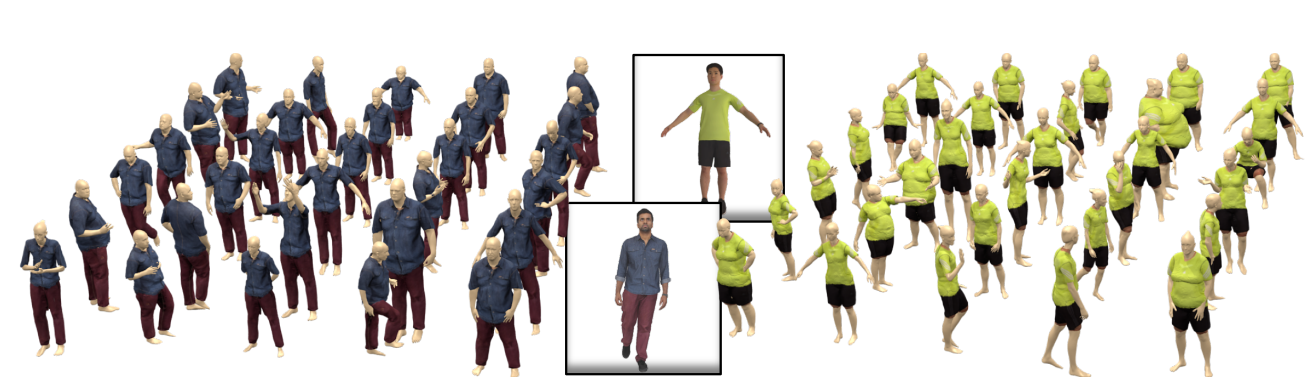
\includegraphics[scale=0.5]{Images/SizerPic/Sizer5.png}
  \caption{Viene utilizzato MGN per l'estrazione dei vestiti da un soggetto sorgente (immagine centrale) e successivamente questi abiti vengono messi su persone arbitrarie in diverse pose grazie a SMPL. I set corrispondono a quello maschile (sinistra) e quello femminile (destra)}
    \label{fig:Sizer5}
\end{figure}

\medskip\medskip\medskip\medskip\medskip\medskip\medskip\medskip\medskip


Gli studi sui vestiti sono tanti, per fare in modo che un essere umano possa indossare virtualmente un abito che si adatti realisticamente ai propri movimenti in base al tipo di tessuto che si vuole rappresentare, bisogna fare un lavoro di processing dal punto di vista della tassellazione non banale.
In queste esperienze si arriva ad avere una mesh poligonale irregolare, di conseguenza una volta ottenuta la segmentazione non è possibile utilizzare separatamente gli abiti rispetto al resto del modello.

\newpage

\subsection{Approcci 3D}

I lavori che partono da scansioni 3D o sequenze di scansioni 3D che sono stati presi in considerazione sono: BUFF, SizerNet e CAPE, ma di seguito vengono illustrati anche due ulteriori metodi rilevanti.

\subsubsection{SPSD}

In “A Layered Model of Human Body and Garment Deformation” (2015 - \url{https://ieeexplore.ieee.org/document/7035823}), viene presentato un framework per l’apprendimento di un modello a tre livelli: forma del corpo umano, posa e deformazione degli indumenti. Il modello di deformazione proposto (Shape and Pose Space Deformation, SPSD) fornisce un controllo intuitivo ed indipendente sui tre parametri, producendo deformazioni naturalistiche sia degli abiti sia del corpo umano. I layer di deformazione della forma e della posa del modello sono addestrati su un ampio dataset di 520 scansioni 3D di 115 soggetti umani (57 uomini e 57 donne) in varie pose (N. Hasler, C. Stoll, M. Sunkel, B. Rosenhahn and H. P. Seidel, "A Statistical Model of Human Pose and Body Shape", Computer Graphics Forum, vol. 28, no. 2, pp. 337-346, 2009.). Il layer della deformazione degli indumenti, invece, è addestrato su sequenze di mesh animate di attori vestiti e si basa su una tecnica per la stima della forma e della postura umana sotto i vestiti. Il contributo chiave di tale articolo è la considerazione delle deformazioni degli abiti come trasformazioni residue tra una mesh di un soggetto svestito ed una della stessa persona vestita.
L'inizializzazione della posa richiede un input manuale.


%\newpage

\subsubsection{BUFF}

In “Detailed, accurate, human shape estimation from clothed 3D scan sequences” (2017 - \url{https://arxiv.org/pdf/1703.04454.pdf}) si parte da scansioni statiche 3Dimensionali, o sequenze di scansioni 3D, e si cercano di stimare posa e forma al di sotto dei vestiti. Se tali scansioni contengono informazioni sul colore, queste vengono usate per dividere i vertici delle scansioni in pelle e indumento, altrimenti tutti i vertici vengono considerati appartenenti ai vestiti. Viene usato il metodo di segmentazione descritto in \url{https://www.researchgate.net/publication/318612942_ClothCap_Seamless_4D_Clothing_Capture_and_Retargeting}. Per rendere uniforme la funzione di costo, viene calcolata prima la distanza geodetica tra un punto e quello del tessuto più vicino, per poi applicare una funzione logistica per mappare i valori della distanza geodetica compresi tra 0 e 1 (Fig. 3 b). Il valore risultante viene propagato ai punti di scansione mediante nearest distance e utilizzato per pesare ogni residuo di scansione. In questo modo, i punti vicini al confine pelle-tessuto hanno un peso decrescente uniforme. Ciò rende effettivamente la funzione non discontinua (smooth) e robusta a segmentazioni imprecise.


\begin{figure}[ht!]
  \centering
  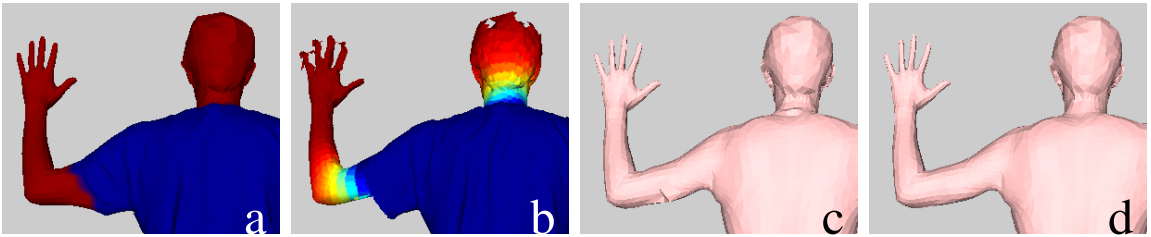
\includegraphics[scale=0.5]{Images/IntroductionPic/BUFF.png}
  \caption{Valore dei pesi dati alla pelle. \\ a) segmentazione ed allineamento (rosso: pelle, blu: vestiti) \\ b) distanza geodetica dal vertice del tessuto più vicino relativo all'allineamento \\ c) risultato 'sbagliato' con collo e braccio non generalizzato \\ d) risultato finale}
  \label{fig:BUFF}
\end{figure}

\medskip

Il dataset BUFF (\url{https://3dmd.com/tag/buff-dataset/}) contiene 11’054 clothed scans ad alta risoluzione con la corrispondente ground truth naked shape per ogni soggetto.

\newpage

\subsubsection{Sizer}

In “SIZER: A Dataset and Model for Parsing 3D Clothing and Learning Size Sensitive 3D Clothing” (\url{https://virtualhumans.mpi-inf.mpg.de/papers/tiwari20sizer/sizer.pdf}) ci si focalizza sulla vestibilità di vestiti virtuali su scansioni 3D del corpo. Gli indumenti interagiscono con il corpo in modo complesso, e la vestibilità è una funzione non lineare di taglia e shape del corpo, per cui simulare tale vestibilità non è banale. Viene introdotto il dataset SIZER (\url{http://virtualhumans.mpi-inf.mpg.de/sizer/}), un dataset di circa 2000 scansioni 3D di 100 persone che indossano 10 tipi di vestiario in taglie diverse (S, M, L, XL), registrazioni sul modello SMPL, scansioni segmentate in tipi di vestiario, categorie di vestiti e taglie.
Con SIZER viene addestrata una rete neurale, SizerNet, che permette di stimare e visualizzare la vestibilità dei vestiti in base alla taglia, la human body shape e l’indumento dati in input. L’addestramento di SizerNet necessita di un mapping tra le scansioni e mesh multi-strato - mesh separate per il corpo e per i capi di sopra e di sotto. Per fare ciò, c’è bisogno di segmentare le scansioni 3D, stimare la body shape senza vestiti e registrare gli indumenti attraverso il dataset ottenuto tramite una feature extraction effettuata mediante i metodi spiegati in “Bhatnagar, B.L., Tiwari, G., Theobalt, C., Pons-Moll, G.: Multi-garment net: Learning to dress 3d people from image” - 2019 http://virtualhumans.mpi-inf.mpg.de/mgn/ - e “ Pons-Moll, G., Pujades, S., Hu, S., Black, M.: ClothCap: Seamless 4D clothing capture and retargeting. ACM Transactions on Graphics 36(4)” - 2017 \url{https://virtualhumans.mpi-inf.mpg.de/papers/ponsmollSIGGRAPH17clothcap/ponsmollSIGGRAPH17clothcap.pdf}.
Dalle mesh multi-livello viene addestrato un codificatore in grado di mappare la mesh data in input ad un codice, ed un decodificatore che prende i parametri della forma del corpo di SMPL, la taglia dei vestiti dati in input e la taglia desiderata, per predire la vestibilità dei vestiti della taglia desiderata. Le scansioni, tuttavia, sono solo nuvole di punti, e analizzandoli (parsing) in una rappresentazione multi-layer al momento del test usando il metodo spiegato precedentemente (nel todo), richiede segmentazione, la quale può avere bisogno di un intervento manuale. Per questo è stata proposta anche ParserNet, la quale mappa automaticamente la registrazione di una singola mesh ad una mesh multi-layer con un solo passo feed-forward. ParserNet non solo segmenta la singola mesh registration, ma riparametrizza la superficie in modo da renderla coerente con i template dei vestiti più comuni.
La rappresentazione multi-layer di ParserNet permette dunque di modificare i vestiti direttamente da una mesh data in input, eliminando la necessità di una segmentazione delle scansioni.
Vengono quindi utilizzate: una rete neurale che predice i parametri relativi alla posa, una per predire i parametri della forma, ParserNet, che fa la segmentazione (riconosce il corpo e i singoli vestiti) e SizerNet, che modifica la taglia dei vestiti: prende in input una mesh 3D e restituisce in output corpi 3D svestiti ad alta qualità, mantenendo l’identità del soggetto.


\begin{figure}[ht!]
  \centering
  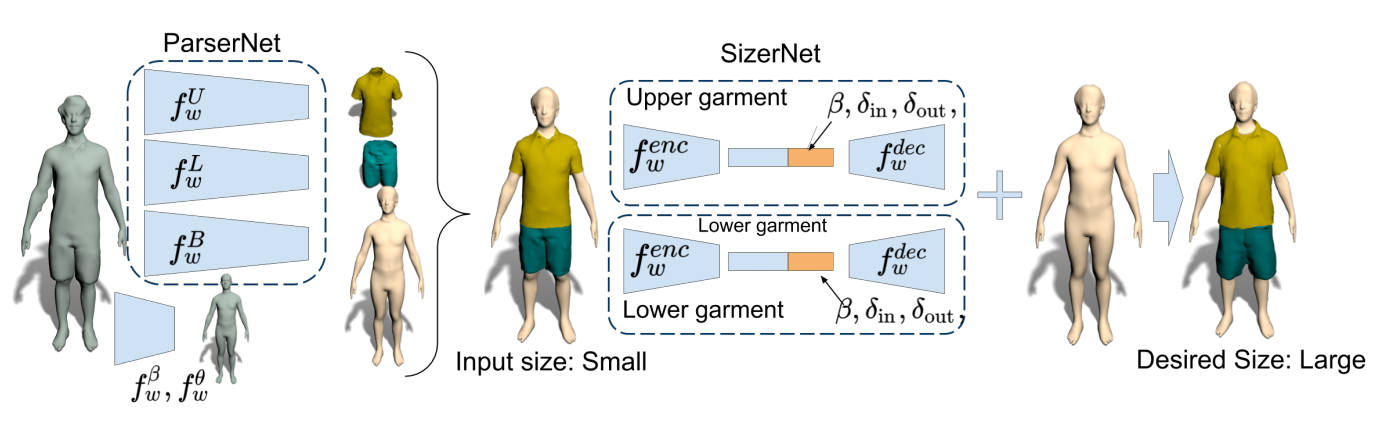
\includegraphics[scale=0.45]{Images/IntroductionPic/Sizer.png}
  \caption{Viene proposto un modello per stimare e visualizzare l'effetto che viene a formarsi vestendo capi condizionati dalla forma e dalla taglia del corpo. Per fare questo viene introdotto ParserNet $(f_{w}^{U}, f_{w}^{L}, f_{w}^{B})$, che prende una mesh precedentemente registrata da SMPL $M(\boldsymbol{\theta}, \boldsymbol{\beta}, \mathbf{D})$ come input e prevede i parametri SMPL $(\boldsymbol{\theta}, \boldsymbol{\beta})$ analizzando gli indumenti 3D ed utilizzando dei modelli predefiniti $T^{g}(\boldsymbol{\beta}, \boldsymbol{\theta}, \mathbf{0})$ prevedendo la forma del corpo che si cela sotto ai vestiti continuando a preservare i dati personali del soggetto. Viene inoltre proposto SizerNet, una rete encoder-decoder $\left(f_{w}^{\mathrm{enc}}, f_{w}^{\mathrm{dec}}\right)$ che ridimensiona il capo $\left(\delta_{\mathrm{in}}, \delta_{\mathrm{out}}\right)$ e lo adatta alla forma del corpo.  }
    \label{fig:Sizer}
\end{figure}

\newpage

\subsubsection{SMPL}
  
MPL, ovvero “Skinned Multi-Person Linear Model (\url{https://files.is.tue.mpg.de/black/papers/SMPL2015.pdf}), si pone come obiettivo quello di rappresentare corpi umani animati realistici che possano compiere diverse pose, deformandosi in maniera completamente naturale mantenendo però la fisionomia e la struttura del corpo umano che tutti noi conosciamo.

  \begin{figure}[ht!]
  \centering
  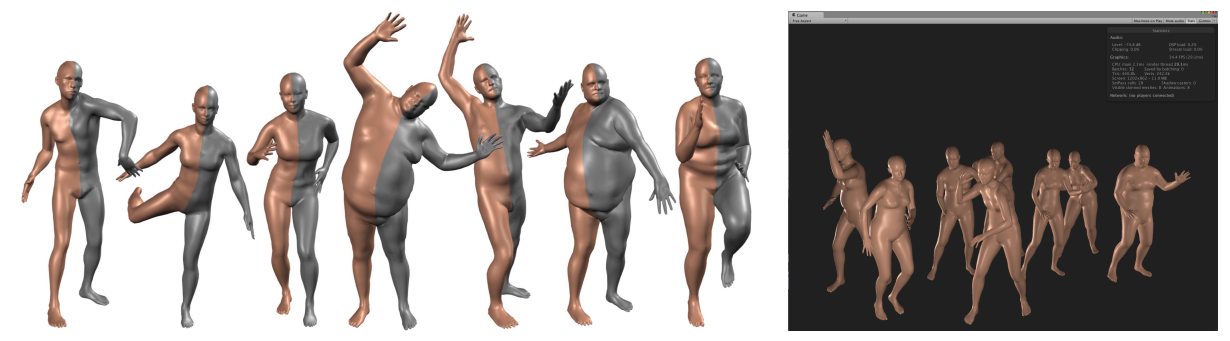
\includegraphics[scale=0.4]{Images/IntroductionPic/SMPL.png}
  \caption{SMPL è un modello realistico appreso della forma e della posa del corpo umano che è compatibile con i motori di rendering esistenti, consente
controllo dell'animatore ed è disponibile per scopi di ricerca. (a sinistra) Modello SMPL (arancione) adatto a mesh 3D della verità a terra (grigio). (a destra) Unità 5.0
screenshot del motore di gioco che mostra i corpi del dataset CAESAR animati in tempo reale.}
  \label{fig:SMPL}
\end{figure}

\medskip

Tali modelli devono essere precisi, facili da implementare, veloci da renderizzare e compatibili con i motori di editor/rendering preesistenti sul mercato. Per realizzare tutto sono necessarie molte blend shapes , molto problematiche da realizzare perché richiedono un enorme sforzo manuale e altrettanto investimento temporale. Per ovviare al problema, la comunità di ricerca scientifica si è concentrata sull’apprendimento di modelli statici come per esempio numerose scansioni dello stesso corpo in pose diverse. Inizialmente si è rivelata un’alternativa molto promettente ma, con l’avanzare delle tecnologie, questo metodo si è rivelato non compatibile con i vari software grafici presenti sul mercato e con i vari motori di rendering che utilizzano i metodi di skinning classici.
SMPL descrive, appunto, un modello del corpo umano che possa rappresentare una vasta gamma di pose, con variazioni dipendenti dalla posa stessa mostrando il funzionamento delle dinamiche dei tessuti molli mantenendo l’efficienza e la compatibilità con i motori di rendering esistenti.
I metodi tradizionali modellano il modo in cui i vertici sono correlati ad una struttura scheletrica sottostante. Il modello più utilizzato è senza ombra di dubbio il “Basic Linear Blend Skinning” (LBS) il quale è si supportato da tutti i game engines, nonché efficiente da renderizzare; sfortunatamente però produce deformazioni delle pose completamente irrealistiche rispetto alle articolazioni umane, producendo i famosi effetti “taffy” e “papillon”

\medskip

\begin{figure}[ht!]
  \centering
  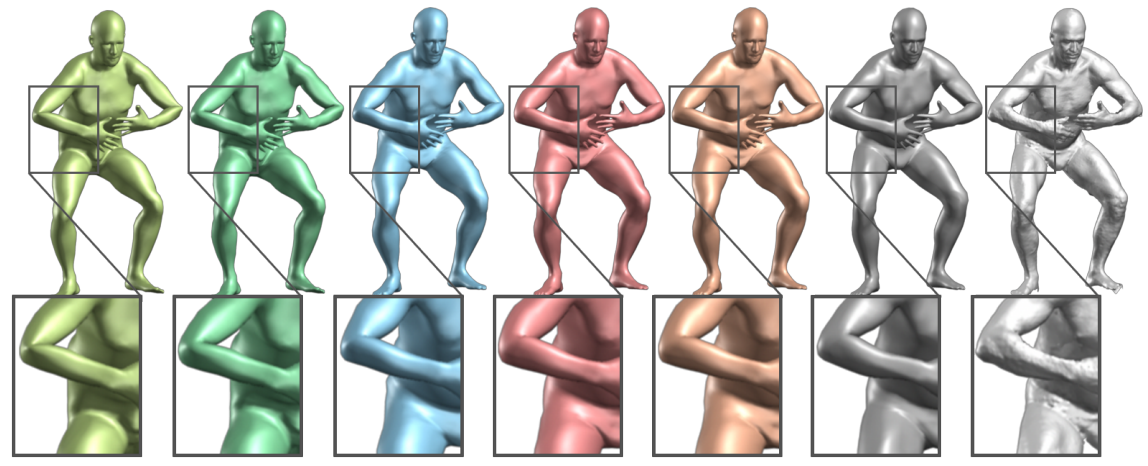
\includegraphics[scale=0.4]{Images/IntroductionPic/SMPL2.png}
  \caption{Modelli a confronto con verità di base. Questa figura definisce la codifica a colori utilizzata nel documento e nel video supplementare.
La mesh all'estrema destra (grigio chiaro) è una scansione 3D. Accanto ad essa (grigio scuro) c'è una mesh registrata con la stessa topologia del nostro modello. Chiediamo come
ben diversi modelli possono approssimare questa registrazione. Da sinistra a destra: (verde chiaro) Skinning blend lineare (LBS), (verde scuro) Skinning blend Dualquaternion (DQBS), (blu) BlendSCAPE, (rosso) SMPL-LBS, (arancione) SMPL-DQBS. Le regioni ingrandite evidenziano le differenze
tra i modelli al gomito destro e all'anca del soggetto. LBS e DQBS producono gravi artefatti su ginocchia, gomiti, spalle e fianchi.
BlendSCAPE ed entrambi i modelli SMPL si comportano allo stesso modo bene nell'adattare i dati.}
  \label{fig:SMPL2}
\end{figure}

\newpage

Un lavoro straordinario è stato dedicato sia ai metodi di skinning che cercano di migliorare questi effetti (Lewis et al. 2000; Wang and Phillips 2002; Kavan and Zˇ ara 2005; Merry et al. 2006; Kavan et al. 2008), sia per migliorare l’apprendimento di modelli corporei altamente realistici dai dati (Allen et al. 2006; Anguelov et al. 2005; Freifeld and Black 2012; Hasler et al. 2010; Chang and Zwicker 2009; Chen et al. 2013).
Nonostante gli enormi sforzi nell’implementazione di metodi, sono rimasti annidati molti problemi tra cui:
\begin{itemize}
\item mancanza di realismo
\item non funzionamento con i pacchetti esistenti
\item non rappresentazione di una discreta varietà di pose
\item non compatibilità con le pipeline grafiche standard
\item richiesto un notevole lavoro manuale
\end{itemize}

Contrariamente agli approcci precedenti, un obiettivo chiave del progetto SMPL è quello di rendere il modello del corpo il più semplice e standard possibile in modo che possa essere ampiamente utilizzato, mantenendo allo stesso tempo il  realismo di modelli basati sulla deformazione appresi dai dati. Nello specifico vengono implementate diverse blend shapes per correggere i limiti dello skinning tradizionale.
Blend shapes per identità, posa e dinamiche dei tessuti molli vengono combinate in modo additivo con un modello di riposo prima di essere trasformate da una blend skin.
Per imparare a riconoscere i vari portamenti del corpo, SMPL utilizza 1786 scansioni in alta risoluzioni con un'ampia varietà di pose.
Viene inoltre utilizzata la PCA (principal component analysis) per imparare i modelli lineari maschili e femminili dal dataset CAESAR (con approssimativamente 2000 scansioni maschili e femminili). 

\medskip

Inizialmente viene registrata una mesh template per ogni scansione e ne viene quindi normalizzata la posa (processo molto importante quando si sta imparando da un modello vertex-based shape).


\medskip

Successivamente viene allenato il modello SMPL in diversi modi e confrontato quantitativamente con un simile modello BlendSCAPE [Hirshberg et al. 2012], allenato anch’esso con gli stessi dati.
I 2 modelli vengono poi valutati qualitativamente con animazioni e quantitativamente utilizzando delle mesh mai viste durante la fase di training.
SMPL e BlendSCAPE vengono adattati a queste nuove mesh e viene fatta un’analisi sugli errori di vertice.
Sono state esplorate principalmente 2 varianti del modello SMPL:
\begin{enumerate}
\item la prima utilizzando LBS (linear blend skinning)
\item la seconda usando DQBS (Dual-Quaternion blend skinning)
\end{enumerate}

\medskip

Risulta che un modello skinned vertex-based come SMPL è molto più accurato rispetto a un modello deformation-based come il BlendSCAPE (avendo svolto la fase di training sugli stessi dati).
Il modello SMPL è stato anche esteso per catturare e modellare la dinamica dei tessuti “molli” adattando il Dyna model [Pons-Moll et al. 2015].
Il risultante modello “Dynamic-SMPL” o DMPL, viene addestrato dallo stesso set di dati di mesh 4D di Dyna. DMPL, a differenza di Dyna, si basa su vertici anziché su deformazioni triangolari. Successivamente vengono calcolati ed analizzati gli errori di vertice tra le mash SMPL e Dyna, e tramite l’utilizzo di PCA viene ridotta la dimensionalità producendo delle blend shapes dinamiche. Un modello di tessuto “molle” viene addestrato sulla base di velocità angolari e deformazioni dinamiche con fatto in [Pons-Moll et al. 2015]. In questo genere di tessuti, la dinamica dipende fortemente dalla forma del corpo; DMPL viene addestrata usando corpi con variabili indici di massa corporea e concentrandosi nel training che dipenda fortemente dai movimenti e pose del corpo stesso.

\newpage

\paragraph{Linear Blend Skinning}~

\medskip

La skin blend lineare è l'idea di trasformare i vertici all'interno di una singola mesh mediante una (blend) di più trasformazioni. Ogni trasformazione è la concatenazione di una "matrice di legame" che porta il vertice nello spazio locale di un dato "osso" e una matrice di trasformazione che si sposta dallo spazio locale di quell'osso in una nuova posizione.
Verrà usata una shader di questo tipo:

\medskip

\begin{figure}[ht!]
  \centering
  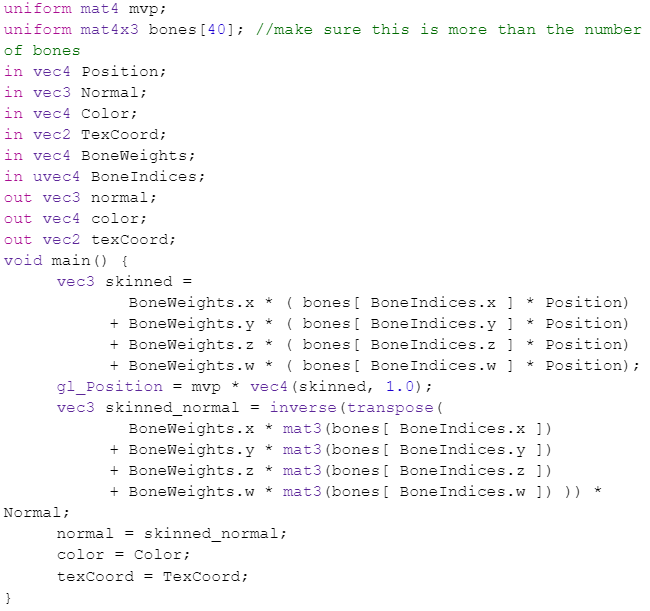
\includegraphics[scale=0.9]{Images/IntroductionPic/LBShape.png}
  \label{fig:LBShape}
\end{figure}

\newpage

\paragraph{Blend Shapes}~

Le Blend Shapes permettono di trasformare la forma di un oggetto in un altro, più nello specifico consentono di trasformarne la superficie stessa.
Per esempio, un uso ricorrente delle Blend Shapes riguarda l’animazione facciale:


\begin{figure}[ht!]
  \centering
  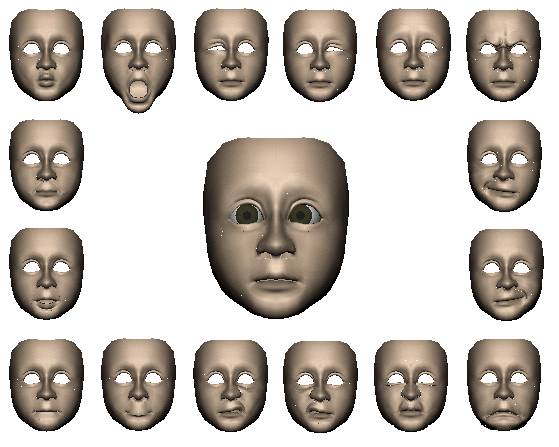
\includegraphics[scale=0.6]{Images/IntroductionPic/BlendShapes.png}
  \caption{Quando viene creata una blend shape, si identificano uno o più oggetti che si vogliono deformare. Gli oggetti utilizzati per “prendere” la forma interessata sono chiamati oggetti target, mentre l'oggetto deformato è chiamato oggetto base.}
  \label{fig:LBShape}
\end{figure}

\subsubsection{CAPE}

CAPE (\url{https://cape.is.tuebingen.mpg.de/media/upload/CAPE_paper.pdf}) è un modello generativo strutturato su grafi a base di reti neurali convoluzionali per la realizzazione di mesh tridimensionali specifiche per l’adattamento dei vestiti al corpo umano. È compatibile con i più famosi modelli che analizzano il corpo umano, come per esempio SMPL,  e può essere generalizzato a particolari pose e movimenti del corpo. È progettato per essere "plug-and-play" per molte applicazioni che già utilizzano SMPL.
Il dataset di CAPE fornisce delle mesh registration nel metodo SMPL quadridimensionali di scansioni relative a persone vestite, insieme a scansioni veritiere delle forme del corpo spoglie di ogni vestito.


\medskip

Per modellare i corpi vestiti, CAPE li fattorizza in due parti: 
\begin{enumerate}
\item corpo con pochi vestiti
\item layer vestito rappresentato come un offset dal corpo
\end{enumerate}

\medskip

Classificando in questo modo, CAPE è in grado di estendere in maniera completamente naturale SMPL ad una classe di tipi di abbigliamento trattando il vestito come una shape aggiuntiva.
Grazie alla rapida diffusione di SMPL, l’obiettivo di CAPE è diventato quello di estendere i metodi implementati da SMPL in maniera coerente agli attuali usi.

\newpage

Come già precedentemente spiegato, SMPL è un modello che fattorizza la superficie del corpo nei parametri forma $(\beta)$ e posa $(\theta)$.
Come mostrato nella figura sottostante (sezione a,b), l'architettura di SMPL inizia con il template di una mesh triangolare $\bar{T}$, definita da $N=6890$ vertici. Dopo aver dato al modello i parametri forma e posa $(\beta, \theta)$, vengono aggiunti al template gli offset 3D corrispondenti a deformazioni dipendenti 

\medskip 

\begin{itemize}
\item dalla forma $\left(B_{S}(\beta)\right)$
\item dalla posa $\left(B_{P}(\theta)\right)$
\end{itemize}

La posa della mesh risultante viene ottenuta usando una funzione di skinning W. Formalmente abbiamo:

\medskip

\begin{equation}
\begin{aligned}
T(\beta, \theta) &=\bar{T}+B_{S}(\beta)+B_{P}(\theta) \\
M(\beta, \theta) &=W(T(\beta, \theta), J(\beta), \theta, \mathcal{W})
\end{aligned}
\end{equation}

\medskip

dove la funzione di sfumatura della pelle $W(-)$ ruota i vertici $T$ della posa a “riposo” intorno ai giunti tridimensionali $J$ (calcolati grazie a $\beta$), li “leviga” linearmente grazie ai pesi di fusione  $W$ e restituisce i vertici della nuova posa $M$. 

\medskip

\begin{figure}[ht!]
  \centering
  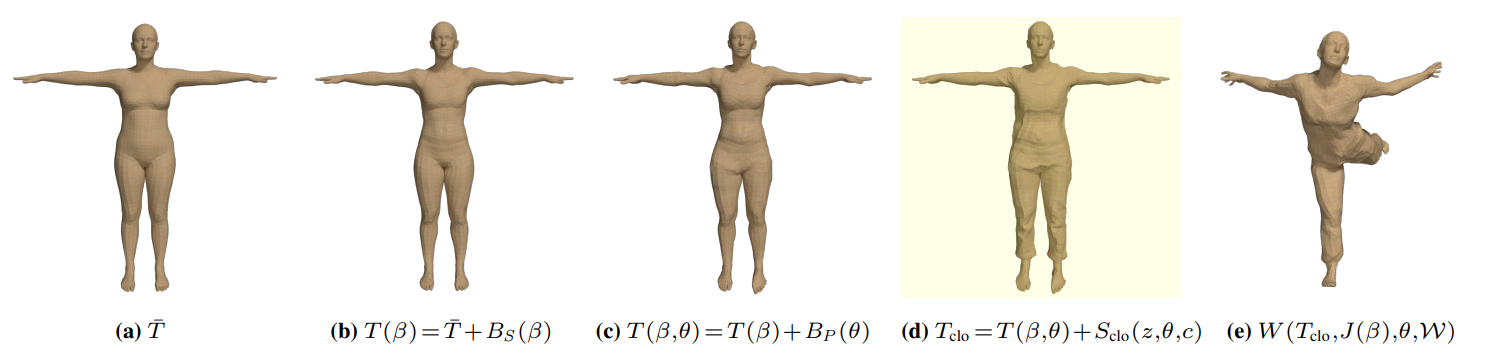
\includegraphics[scale=0.4]{Images/IntroductionPic/CAPE.png}
  \caption{Il contributo principale viene evidenziato dallo sfondo giallo.\\
  Partendo da SMPL, CAPE (a) aggiunge linearmente gli offset forniti da (b), la forma del corpo individuale $(/beta)$ e (c) la posa $(/theta)$; da notale da deformazione sui fianchi e sui piedi per via della posa. (d) Viene inoltre aggiunto uno strato di abbigliamento c e una variabile di forma z. (e) i vertici vengono computati usando l'equazione di skinning di SMPL.}
  \label{fig:CAPE}
\end{figure}

\medskip

SMPL aggiunge dei livelli (strati) di deformazione lineare ad uno strato iniziale composto dalla posa “standard” del corpo.
Successivamente, CAPE definisce l’abbigliamento come  un livello extra di offset dal corpo e lo aggiunge sopra alla mesh realizzata da SMPL, come in Fig. 2 (d).

\newpage

\paragraph{Architettura della rete}~
\medskip

Come mostrato nell'immagine sottostante, il modello è costituito da un generatore
G con architettura encoder-decoder e discriminatore D. Vengono inoltre utilizzate reti ausiliarie C1, C2 per gestire il problema del condizionamento. La rete è differenziabile ed è trainata end to end.

\begin{figure}[ht!]
  \centering
  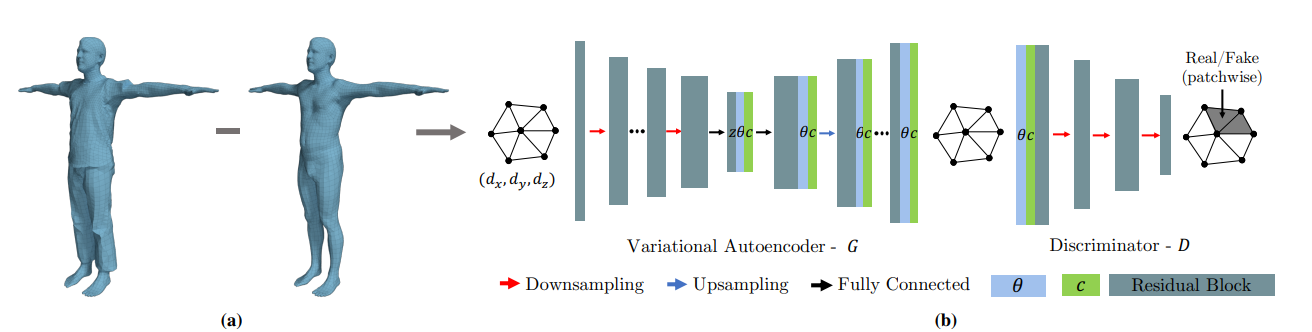
\includegraphics[scale=0.4]{Images/IntroductionPic/CAPENetwork.png}
  \caption{(a) calcola gli spostamenti dai dati di scanzione sottraendo la minima forma del corpo dalla mesh del corpo vestito (b) }
  \label{fig:CAPENetwork}
\end{figure}


Per semplicità, in questa sezione verrà utilizzata la seguente notazione.

\medskip

$x$: i vertici $\nu_d$ del grafo di spostamento in ingresso; \\
$X$: vertici del grafo ricostruito;\\
$\theta$ e $c$: la posa ed il
vettore di condizionamento in base al capo\\
$z$: il codice latente.

\medskip

\textbf{Generatore di grafici}. Viene costruito il generatore di grafi seguendo una rete di tipo VAE-GAN. Durante l'allenamento, un encoder Enc(·)
prende lo spostamento x, estrae le sue caratteristiche attraverso più strati convoluzionali del grafico e lo mappa sul codice latente a bassa dimensione z. Un decoder viene addestrato per ricostruire il grafico di input $\hat{x}=D \operatorname{ec}(z)$ da z. Sia l'encoder che il decoder sono reti neurali feed-forward costruite
con strati convoluzionali mesh. I livelli lineari sono usati alla fine dell'encoder e all'inizio del decoder.

\medskip

L'impilare i livelli convoluzionali provenienti dal grafico genera una perdita di features negli strati più profondi. Questo è un gravissimo problema, soprattutto nell'ambito del clothing generation perchè alcuni dettagli, come per esempio le pieghe, tendono a scomparire.Pertanto, vengono migliorati gli strati di convoluzione del grafico standard con connessioni residue, che consentono l'uso di caratteristiche di basso livello da quello di input, se necessario.

\medskip

Al momento del test, l'encoder non è necessario. Invece, z viene campionato dalla distribuzione a priori gaussiana e dal decodificatore
funge da generatore di grafici: $G(z) = Dec(z)$.

\medskip

\textbf{Discriminatore Patchwise}. Per migliorare ulteriormente i dettagli nella fase di ricostruzione, viene introdotto un discriminatore patchwise D per i grafici, che ha mostrato successo nel dominio dell'immagine.

Invece di guardare l'intero grafico generato, il discriminatore classifica solo se la patch è vera o falsa in base alla sua struttura locale. Intuitivamente questo incoraggia il discriminatore a concentrarsi solo sui
dettagli più raffinati e per quanto riguarda la forma 'globale', se ne occupa la reconstruction loss.

\medskip

Viene implementato il grafico patchwise-discriminator utilizzando quattro grafici di convoluzione-sottocampionamento a
blocchi. Successivamente viene aggiunto una perdita reale/fasulla discriminante per ciascuno dei vertici di output.  Questo abilita il discriminatore
a catturare una patch di nodi vicini nel grafico ricostruito e classificarli come reali / falsi.

\medskip

\textbf{Modello condizionale}. Si condiziona la rete con bodypose $\theta$ e abbigliamento di tipo c. I parametri di posa SMPL sono
nella rappresentazione asse-angolo e sono difficili da apprendere per la rete neurale.
Pertanto vengono trasformati i parametri di posa in matrici rotazionali usando l'equazione di Rodrigues.
Entrambe le condizioni v engono prima passate attraverso una piccola rete di incorporamento completamente connessa, $C_{1}(\theta), C_{2}(c)$, rispettivamente, in modo da bilanciare la dimensionalità di apprendimento delle features del grafico e di condizionamento.

\medskip

Si sperimenta, inoltre, diversi modi di condizionare il generatore di mesh: 

Concatenazione nello spazio latente; aggiungere le features delle condizioni alle features del grafico in tutti i nodi del generatore; e la combinazione dei due. Risulta che la strategia combinata funziona meglio in termini di capacità di rete e di effetto del condizionamento.


\paragraph{Ricostruzione di persone 3D}~

La ricostruzione di esseri umani 3D da immagini e video 2D è un classico problema di visione artificiale.
La maggior parte degli approcci generano mesh del corpo 3D dalle immagini, ma non dai vestiti.
Questo tipo di approccio ignora completamente dettagli delle immagini che potrebbero essere utili ai fini dell’obiettivo stesso.
Per ricostruire i corpi con i vestiti addosso, i più famosi metodi utilizzano rappresentazioni di profondità volumetriche  o biplanari per modellare il corpo e gli abiti nel loro insieme.
Un altro gruppo di metodi si basa sul SMPL.
Rappresentano l'abbigliamento come uno strato sfalsato rispetto al corpo sottostante come proposto in ClothCap (gruppo 2 nella Tabella 1).

\paragraph{Modelli parametrici per corpi e abiti 3D}~

I modelli statistici tridimensionali del corpo umano ricavati dalle scansioni 3D catturano la forma e la posa, rendendoli un elemento fondamentale per molteplici applicazioni.
Nella maggior parte dei casi, tuttavia, le persone sono vestite quando questi modelli non rappresentano l’abbigliamento stesso.
Inoltre, mentre ci muoviamo, i vestiti cambiano forma producendo pieghe che a loro volta possono mutare in molti modi diversi.
Sebbene esistano modelli di abbigliamento appresi da dati reali, pochi di questi si adattano a pose non comuni. Ad esempio, Neophytou e Hilton apprendono un modello basato sulla stratificazione degli indumenti sulla base di SCAPE da sequenze dinamiche, anche se la generalizzazione a nuove pose non è ancora stata dimostrata.
Un approccio concettualmente diverso deduce i parametri di un modello di abbigliamento da sequenze di scansioni tridimensionali.
In questo caso è possibile generalizzare a nuove pose creando, però, il grave problema dell’interferenza e, a differenza di CAPE, il simulatore fisico risultante non è differenziabile rispetto ai parametri stessi.

\medskip

Il dataset CAPE è facilmente scaricabile, sono approssimativamente 49GB.
Per ottenere i dataset di Buff (\url{https://arxiv.org/pdf/1703.04454.pdf}) e SIZER bisogna necessariamente contattare gli owners.
Per Buff bisogna inviare una email seguendo le istruzioni del seguente link \url{http://buff.is.tue.mpg.de/downloads}. Per quanto riguarda SIZER, invece, qui c'è un form da compilare \url{https://docs.google.com/forms/d/e/1FAIpQLSddBep3Eif1gI-6IhaZybBDoR-_H_QW1NST0JV5vviauvPNTA/viewform}, oppure si può inviare una mail a \url{gtiwari@mpi-inf.mpg.de} per ottenere sia il dataset che il modello, come indicato qui \url{https://github.com/garvita-tiwari/sizer}.

\medskip

La cattura, ricostruzione e la modellazione di abiti sono 3 punti che sono stati ampiamente studiati negli ultimi decenni.
La tabella 1 mostra i più famosi metodi degli ultimi anni categorizzati in due classi principali: (1) metodi di ricostruzione e cattura e (2) modelli parametrici, dettagliati come segue.

\medskip

\begin{figure}[ht!]
  \centering
  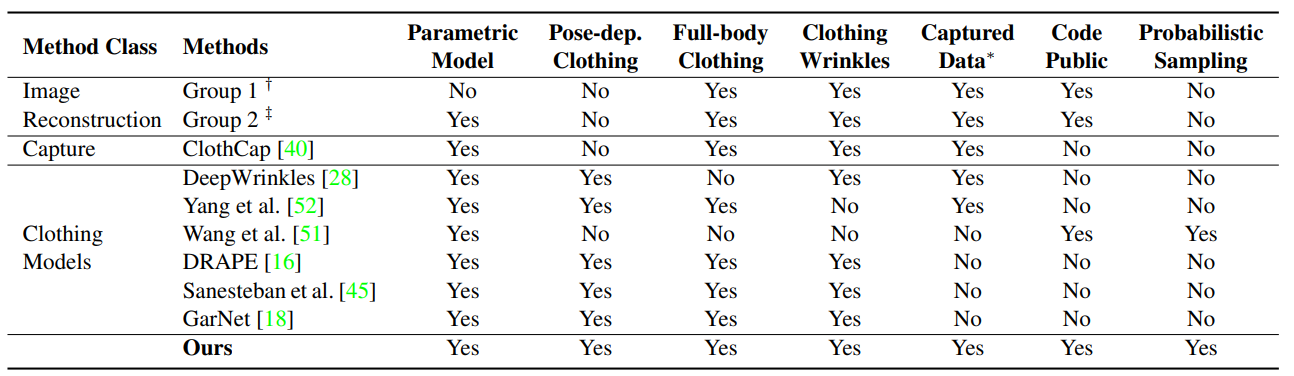
\includegraphics[scale=0.4]{Images/IntroductionPic/CAPETabel.png}
  \caption{Selezione di metodi correlati. Esistono due principali classi di metodi di abbigliamento 3D: (1) metodi di ricostruzione e acquisizione basati su immagini e (2) abbigliamento
modelli che prevedono la deformazione in funzione della posa. All'interno di ciascuna classe, i metodi differiscono in base ai criteri nelle colonne.}
  \label{fig:CAPETabel}
\end{figure}

\medskip

\subsubsection{ClothCap}

In “ClothCap: Seamless 4D Clothing Capture and Retargeting” 

(\url{https://virtualhumans.mpi-inf.mpg.de/papers/ponsmollSIGGRAPH17clothcap/ponsmollSIGGRAPH17clothcap.pdf})

\medskip

L’idea di questo metodo, invece, riguarda un approccio data-driven alla cattura dei vestiti (ClothCap); processando abbigliamento dinamico vestito su persone da scansioni quadridimensionali in modo da poter essere computato in maniera più semplice dei tradizionali metodi e applicato su avatar virtuali.

\medskip

Viene catturata la geometria dell’abito su un corpo in movimento, viene stimata sia la forma del corpo che la sua morfologia sotto i vestiti per poi segmentare ed estrarre i vari capi.
I nuovi capi catturati in questo modo vengono assegnati successivamente a nuove persone, anche con pose differenti.

\medskip

Per fare ciò, viene sviluppato un modello multi-parte orientato alle mesh dimostrando come segmentare, rintracciare e recuperare la forma di un capo a partire da sequenze di scansioni tridimensionali.

\medskip

\begin{figure}[ht!]
  \centering
  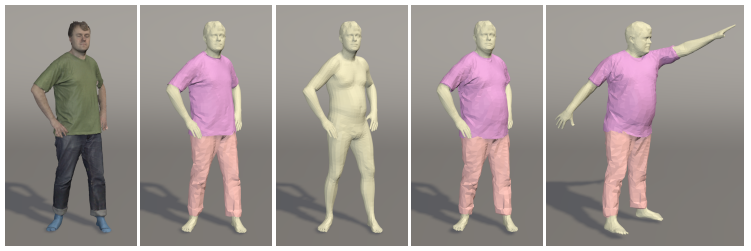
\includegraphics[scale=0.5]{Images/SizerPic/Sizer6.png}
  \caption{Da sinistra a destra: (1) Un esempio di scansione con texture 3D che fa parte di una sequenza 4D. (2) Il modello di mesh allineato in più parti, sovrapposto al
corpo. (3) La forma minimamente vestita (MCS) stimata sotto i vestiti. (4) Il corpo irrobustito e vestito con gli stessi abiti. Si noti che l'abbigliamento
si adatta in modo naturale alla nuova forma del corpo. (5) Questa nuova forma del corpo si pone in una posa nuova, mai vista. Questo illustra come ClothCap supporta una gamma di
applicazioni relative all'acquisizione, alla modellazione, al retargeting, alla posa e alla prova di abbigliamento}
    \label{fig:Sizer6}
\end{figure}

\medskip

I metodi di cattura esistenti soffrono di bassa risoluzioni, forme statiche, troppa semplicità nei movimenti del corpo, cattura di solo un capo di abbigliamento o la non completa segmentazione dei vestiti.
Conseguentemente, i problemi chiave da risolvere includono l’acquisizione di alta qualità, la segmentazione, il tracciamento della forma e della superficie così come la stima della morfologia del corpo e come questo stia posando.

\medskip

Come input, viene data una nuvola di punti (con texture).

\medskip

La rappresentazione multi-mesh è consistente con il modo in cui l’abito viene indossato, modellando e adattando il continuo cambiamento di visibilità delle superfici del vestito nel tempo.
Inoltre permette di affrontare i problemi di segmentazione e tracciamento in un quadro coerente. In questo modo vengono segmentati automaticamente gli abiti dalle scansioni quadridimensionali usando informazioni sia riguardanti l’aspetto che la forma (Fig. 1 (2)) utilizzando un campo casuale di Markov 

\url{https://www.dsu.univr.it/documenti/Tesi/allegato/allegato517081.PDF}

\medskip

Dati gli abiti segmentati, viene adattato un set di modelli multiparte basati a mesh alle scansioni, mettendoli in corrispondenza nel tempo e stimando così la forma sottostante del vestito in forma minimale

\medskip

La filosofia di questo metodo sposta l’attenzione dalla simulazione alla cattura dei vestiti.
Le mesh dei vestiti estratte automaticamente sono naturalmente associate ad un modello corporeo articolato sottostante (SMPL (Loper et al. 2015)).
Grazie a questa tecnologia si è in grado di cambiare la morfologia del corpo come mostrato in (Fig. 1 (4)), oppure trasferire direttamente gli indumenti ad un nuovo corpo in maniera completamente automatica.
è vero che l’acquisizione del modello riguardante le pieghe non è completamente realistico; tuttavia l’aspetto visivo ottenuto è più che sufficiente per molte applicazioni try-on.


\medskip

In sintesi, ClothCap getta le basi per la modellazione degli abiti, affrontando problemi complessi relativi alla segmentazione e tracciamento di scansioni quadridimensionali.
In maniera più dettagliata, contribuisce a 
\begin{itemize}
\item metodo automatico per segmentare le sequenze di scansioni tridimensionali sfruttando un modello corporeo
\item un metodo di tracciamento del modello multi-mesh
\item una tecnica per riorientare il tessuto in maniera dinamica ad una nuova morfologia corporea
\end{itemize}


\medskip

L’intero metodo viene dimostrato estraendo diverse tipologie di abiti tra cui pantaloni lunghi, t-shirt e pantaloncini su un’ampia varietà di persone mentre eseguono movimenti non banali (complessi). Viene inoltre dimostrato che il metodo funziona per le gonne pur avendo una diversa topologia rispetto al corpo.

\medskip

\begin{figure}[ht!]
  \centering
  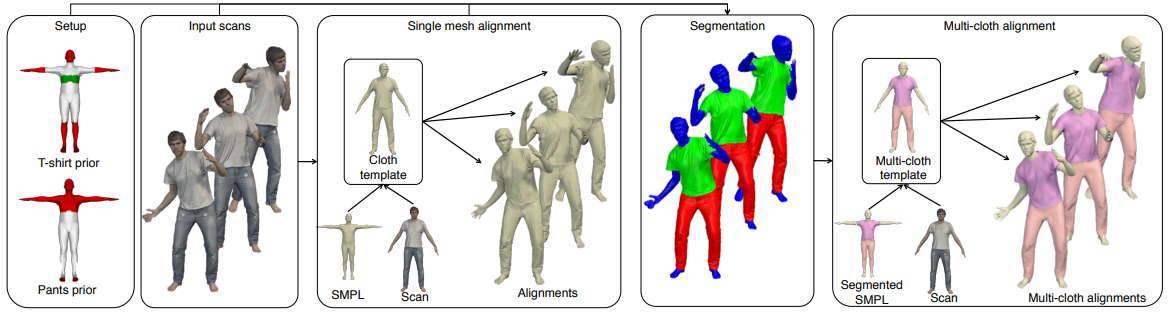
\includegraphics[scale=0.5]{Images/SizerPic/Sizer7.png}
  \caption{Sono necessari tre passaggi principali per ottenere allineamenti multitessuto: allineamento mesh singola, segmentazione della scansione e allineamento multitessuto. Multi-tessuto
gli indumenti di allineamento possono essere facilmente retargettati a nuove forme.}
    \label{fig:Sizer7}
\end{figure}

\medskip

ClothCap si basa su quattro steps principali:

\medskip

\begin{itemize}
    \item \textbf{\textit{Step 0: Installazione}}. Per catturare una specifica classe di abiti è necessario definire il numero di capi “Ngarm”  e istanziare una priorità spaziale relativamente bassa per intuire in quale parte del corpo gli abiti potrebbero trovarsi. Questo processo è molto grezzo e conseguentemente facile da realizzare. Inizialmente vengono trattati vestiti la cui topologia è facilmente mappabile al corpo per poi venire esteso ad un più ampio campo di vestiti con topologie via via più complicate come per esempio le gonne.
    Come modello del corpo viene utilizzato l’SMPL. (Loperet al. 2015).
    Nello specifico, per un soggetto, viene stimata una MCS (minimally clothed shape) ovvero la morfologia approssimativa del soggetto senza vestiti.
    L’MCS potrebbe essere stimato utilizzando una tecnologia esistente (Zhang et al. 2017) ma, dal momento che ClothCap acquisisce scansioni quadridimensionali dal soggetto, l’acquisizione di un’ulteriore scansione per inquadrare gli abiti “di base” richiederebbe minimo sforzo a livello computazionale e tempistico. Quindi viene allineato il modello del corpo insieme alla scansione dei vestiti basilari per ottenere l’ MCS. Infine ClothCap assume che tutte le sequenze di scansione partano (più o meno) con una posa alla “A”.
    \item \textbf{\textit{Step 1: Segmentazione}}.
    Le scansioni quadridimensionali includono geometria e informazione riguardante il colore e, ovviamente, contengono anche rumore e mancanza di dati. Risulta, quindi, difficile segmentare queste scansioni grezze pertanto il problema viene analizzato in due sottoproblemi:
    \begin{itemize}
        \item \textbf{\textit{Step 1a: Allineamento a mesh singola}}. Come primo passo viene allineato alle sequenze scansionate il modello del corpo umano fornito da SMPL. Successivamente ClothCap deforma il modello in modo da adattarlo al meglio ai dati osservati e inizializzare ciascun frame con il risultato del frame precedente. L’output di questo step è una sequenza registrata a bassa risoluzione di meshes.
        \item \textbf{\textit{Step 1b: Segmentazione}}. Attraverso l’utilizzo combinato della priority segmentation e un campo casuale Markoviano è possibile segmentare ogni frame della sequenza. Ciò fornisce una segmentazione sia dei singoli allineamenti della mesh sia una segmentazione basata sui vertici delle scansioni. Quindi grazie all’allineamento segmentato della singola mesh del primo frame (che, come citato sopra, si trova approssimativamente in una posa ad “A”) è possibile definire un template che determini la topologia del capo (ma non la geometria). Infine vengono scartati gli allineamenti della singola mesh.
        
        
    \end{itemize}
    \item \textbf{\textit{Step 2: Allineamento multitessuto}}.
    Il template segmentato dell’abito viene deformato in	modo da adattarsi alla scansione segmentata del primo fotogramma in modo da ottenere un modello multitessuto che è in grado di acquisire sia la topologia che la geometria dei capi e del corpo umano. Con questo tipo di allineamento ogni vestito viene tracciato per combaciare con i dati della scansione segmentata. Questa ottimizzazione implementa un parametro per regolarizzare i bordi del capo come per esempio nelle braccia, sul collo, nella vita e nelle caviglie. Inoltre un ulteriore parametro viene dedicato allo smoothing degli abiti. Questo step genera multi tessuti allineati alle scansioni, ovvero deformazioni del template multitessuto originale. Ne conclude che ogni abito in ogni fotogramma è allineato ad un template comune.
    \item \textbf{\textit{Step 3: Reindirizzamento}}. Per prima cosa bisogna considerare la sorgente di una persona che si sta muovendo con abiti che vogliamo reindirizzare.
    Da questa sequenza viene stimato l’MCS e computato un allineamento multitessuto; questo, però, non è sufficiente per l’operazione di reindirizzamento.
    Nella fase di preparazione viene stimata la morfologia di una persona svestita in un determinato lasso di tempo che potrebbe discostarsi dal MCS e viene stimato come il vestiario si possa adattare a questa nuova forma del corpo nella posa a “T”. Questa operazione viene svolta per ogni singolo fotogramma nella sequenza sorgente.
    Il reindirizzamento di un capo prevede 2 steps:
    \begin{itemize}
        \item preparazione
        \item vestizione 
    \end{itemize}
    
\end{itemize}



\medskip

\begin{figure}[ht!]
  \centering
  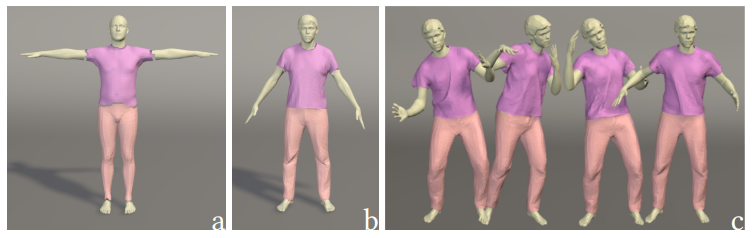
\includegraphics[scale=0.5]{Images/SizerPic/sizer8.png}
  \caption{modello di tessuto segmentato automaticamente: definisce il
solo topologia dell'indumento; cioè, quali vertici appartengono a ciascuna parte di stoffa. (b)
il modello multi-tessuto acquisisce sia la geometria che la topologia. Questo è calcolato
per ogni nuovo soggetto e capo e cattura la geometria di ciascuno
indumento. (c) gli allineamenti multi-tessuto sono deformazioni del multi-telo
modello per adattarsi a ogni fotogramma della sequenza.}
    \label{fig:Sizer8}
\end{figure}

\medskip

\newpage





























 








